\chapter{Simulation and Reconstruction}
\label{ch:Simulation}

% Notes: Should I put in how many events are simulated?

This chapter presents details on the simulation of various physics processes and the reconstruction of physics objects for both simulated events and data events.  

\section{Simulation of pp Collisions}
To draw conclusions from ATLAS experimental data it is necessary to make accurate theoretical predictions about the processes being searched for.  Having accurate background models can help identify when a data signal is behaving in a way that might suggest new physics.  Due to the stochastic nature of particle physics collisions and interactions, it is not practical to create exact predictions.  Instead the ATLAS experiment uses Monte Carlo (MC) simulations to model physical behaviors.  MC simulations are done by repeated random sampling of possible physical processes that can occur at any given time to a particle.  The possibilities change based on factors such as particle energy and particle environment.  A flow chart for the entire simulation chain is shown in Figure \ref{fig:SimMCFlow}. 

\begin{figure}[h!]
	\centering
	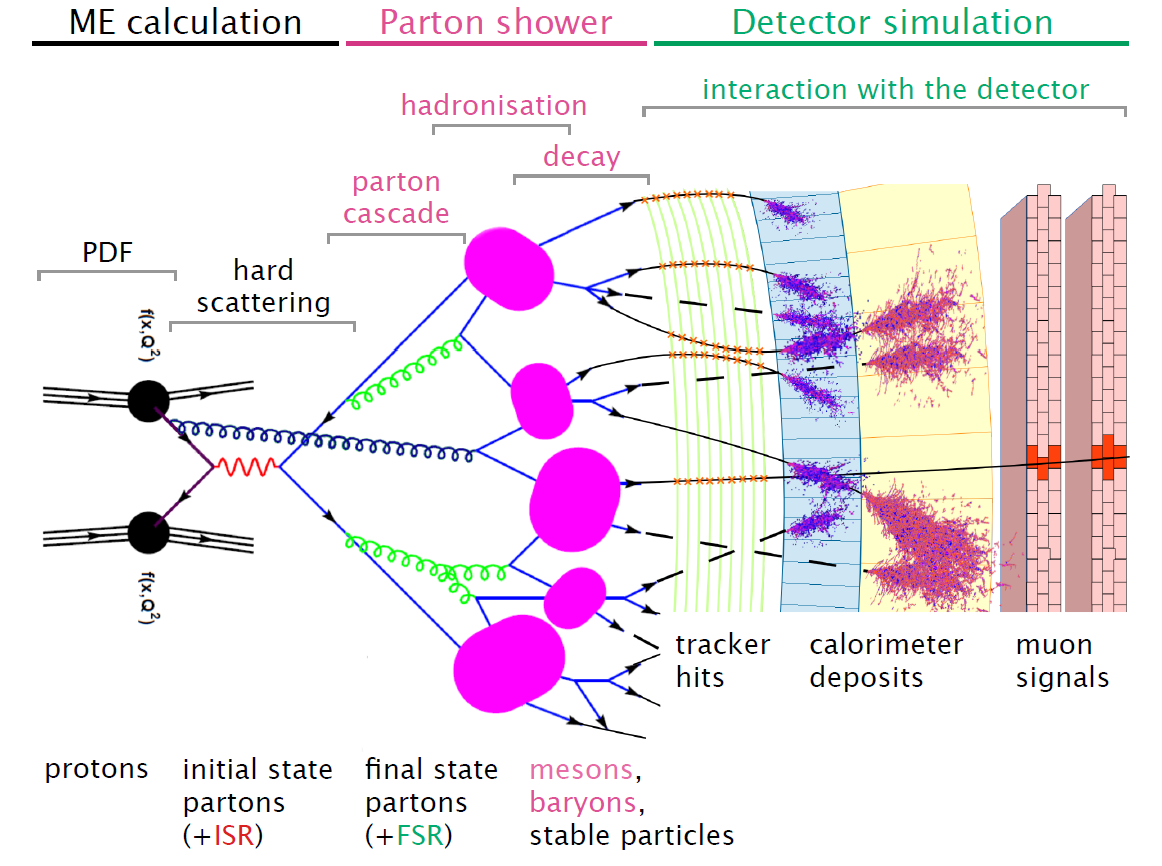
\includegraphics[width=\columnwidth]{../ThesisImages/Simulation/MCFlow.png}
	\caption[A pictoral view of the different steps for the creation of a MC event.]{A pictoral view of the different steps for the creation of a MC event\cite{MaxThesis}.
	}
	\label{fig:SimMCFlow}
\end{figure}

\subsection{ Matrix Element Calculation and Parton Distribution Functions}

Particle interactions at LHC energies do not involve the entire proton.  The constituent partons that create the proton (the two up quarks, down quark, and the sea of gluons) are what interact in any given event.  The gluons create many virtual quark-antiquark pairs which can interact as well.  The valence quarks, the two up quarks and the down quark that make up the proton, are the major portion of interacting partons at low energies, mainly inelastic interactions.  At LHC energies deep inelastic scattering is possible and the sea quarks play a more dominant role.  Proton structure is described by a Parton Distribution Function (PDF) which gives the probability of finding any parton with a particular momentum fraction, shown in Figure \ref{fig:PDF}.

\begin{figure}[h!]
	\centering
	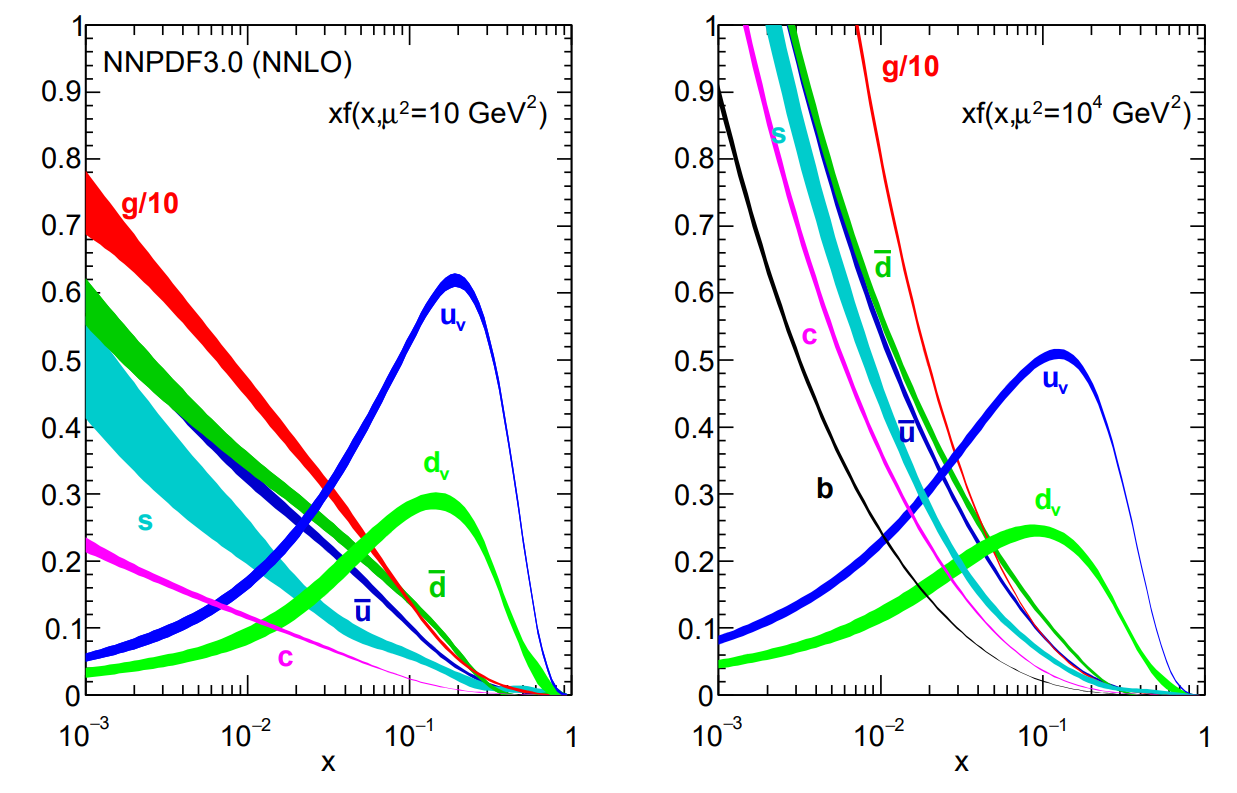
\includegraphics[width=\columnwidth]{../ThesisImages/Simulation/PDF.png}
	\caption[The bands are the momentum fraction, $x$, times the unpolarized parton distribution function obtained in NNLO NNPDF3.0 global analysis at scales $\mu^2= 10$ GeV and $\mu^2 = 100 \text{ GeV}^2$.]{The bands are the momentum fraction, $x$, times the unpolarized parton distribution function obtained in NNLO NNPDF3.0 global analysis at scales $\mu^2= 10 \text{ GeV}^2$ and $\mu^2 = 100 \text{ GeV}^2$\cite{PDG2018}.
	}
	\label{fig:PDF}
\end{figure}
The PDFs and hard scattering processes are included in the calculation of the Matrix Elements (ME) of any interaction.  Hard scattering processes can be descibed by Feynman diagrams, a representation of their amplitudes.  Combining the PDFs and hard scattering amplitudes gives the probability of a particular interaction occuring.  Calculation of the MEs is the first stage of simulation and is done to a specified order in perturbation theory: leading order (LO), next-to-leading order (NLO), etc.  Higher order calculations lead to more accurate predictions but grow exponentially in complexity making them harder to calculate both theoretically and computationally, often restricting how accurately a process can be simulated.  

\subsection{Parton Shower Calculation}
The next stage of simulating an event is the parton shower.  These parton shower calculations deal with the quantum chromodynamic processes.  In any interaction the particles that carry color can spontaneously emit gluons which can go on to create more gluons or quark-antiquark pairs.  Depending on when this happens in the hard scattering process it is called initial state radiation (ISR) or final state radiation (FSR).   The hard scattering partons as well as any additional radiated particles are used as inputs to parton shower calculations which determine how the quarks and gluons proceed through to the final state particles seen in the detector.  This includes calculation of hadronization processes and futher decay processes into the final state particles.

\subsection{Detector Simulation}
The final stage of creating an MC event is the detector simulation.  The information from the event generators are processed using \textsc{geant4}\cite{Geant4} and a detailed model of the ATLAS detector.  \textsc{geant4} simulates how various particles propagate through and interact with the material properties of the detector and where they leave energy which would then be measured by the ATLAS detector in an actual event.  The result of this MC event construction flow is a collection of simulated data that is similar in structure to actual data collected using the ATLAS experiment.  The energy deposits in both MC and real data are combined using the same software used for physics object reconstruction.  For MC events this allows for comparison between the physics object reconstruction and the truth record, or the types of particles fed into the detector simulation.

\subsection{Monte Carlo Generators Used for LHC Physics}

A variety of different MC generators are used in the creation of simulated events.  Different generators specialize in simulating different physics processes to various levels of precision (e.g., LO vs. NLO). The MC generators used in this search are summarized in this section.

\textsc{MadGraph} aMC@NLO\cite{MadGraph}: An amplitude and event generator at LO and NLO for hard processes.  Extendable to various models including effective field theory (EFT) models used in BSM searches.  This generator is used to create the signal events searched for in this dissertation and discussed in Section \ref{Sec:MG5Sig}. 

\textsc{powheg}\cite{Powheg1,Powheg2}: \textbf{Po}sitive \textbf{W}eight \textbf{H}ardest \textbf{E}mission \textbf{G}enerator is an NLO event generator that can be interfaced with other generators (i.e. \textsc{pythia}) for showering.

\textsc{pythia}\cite{Pythia8}: A generator used most often for QCD final state hard processes and showering.  It is commonly interfaced with other generators for showering within the ATLAS detector.

\textsc{sherpa}\cite{Sherpa11,Sherpa22}: A multi-parton LO generator with an emphasis on merging ME and Parton Showering.

A common event file format developed at the Les Houches Accords\cite{Alwall:2006yp} makes it possible for these generators to be interfaced in a straightforward way, typically with \textsc{pythia} for showering.  This allows a specialty generator to be created and used to generate hard processes and then simulate the rest of the event with common showering generators that might lack the ability to simulate the process in question.



%%%%%%% FCNC Generation
\section{Creation of Flavor-Changing Neutral Current Signal Events}
\label{Sec:MG5Sig}
To create simulated signal events the typical Standard Model models must be extended to include higher-order terms.  A Universal FeynRules Output (UFO\cite{UFO}) model was created to include dimension-6 operators(\cite{Dim6TermsOld, Dim6Terms}).  These individual operators are turned on for the specific final state being produced.  The original operators can be reduced to a minimal set of coupling to anomalous final states (i.e., FCNC final states)\cite{TopCouplingsAguilarSaavedra}, used for event production.  This effective field theory method of signal production is beneficial as it allows for production of signal events that are not dependent on any particular BSM model.  This method of including dimension-6 effective operators can be used to produce any of the top FCNC channels, for example in the $t\rightarrow qZ$ process\cite{FCNCtqZ} and $t\rightarrow qH$\cite{UFOModel}.

\subsection{FCNC Events Produced With MadGraph5 aMC@NLO}

Signal events have been produced using MadGraph5 aMC@NLO following the work of Degrande et al.\cite{Degrande:2014tta}.  Before official ATLAS datasets can be produced and the entirety of the event reconstructed through the ATLAS detector, validation of the model must be performed.  10,000 events were produced locally at truth level for each decay channel to compare the kinematics of produced events in $t\bar{t}\rightarrow bWq\gamma$ to the kinematics of official production $t\bar{t}$ events. 

\begin{figure}[h!]
	\centering
	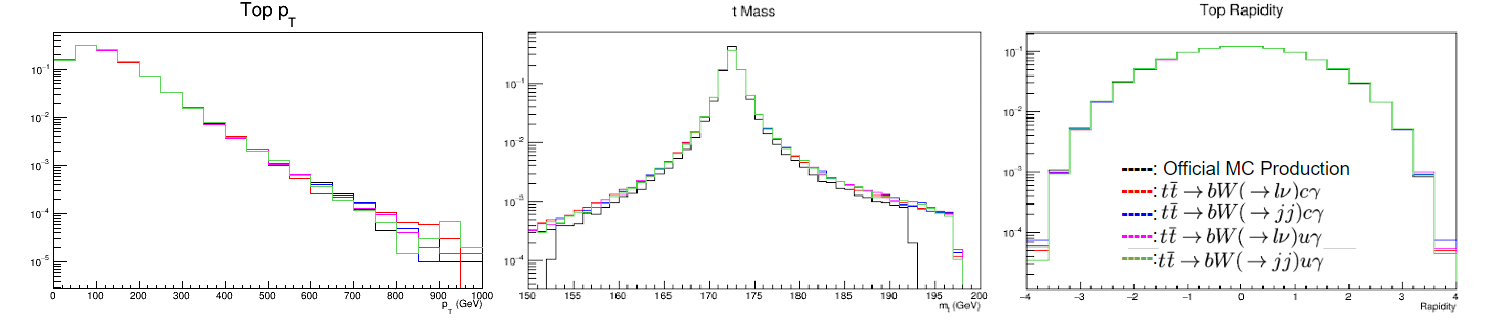
\includegraphics[width=\columnwidth]{../ThesisImages/FCNCValidation/singleTops.png}
	\caption{ Normalized kinematics ($p_T$, $m_t$, and $y_t$) of individual top quarks produced by the model for each FCNC final state search and an official $t\bar{t}$ sample.
	}
	\label{fig:randomfinal1}
\end{figure}


The minimal couplings mean there is one scalar coupling introduced for each decay mode, $t\rightarrow c\gamma$ and $t\rightarrow u\gamma$.  All possible final states are shown in the figures in this section: the leptonic and hadronic decays of the W boson from the top quark that decays through the typical Standard Model decay mode $t\rightarrow bW$.  Figure \ref{fig:randomfinal1} shows individual top quark truth information while the validation of the $t\bar{t}$ system kinematics are shown in Figure \ref{fig:randomfinal2}.

\begin{figure}[h!]
	\centering
	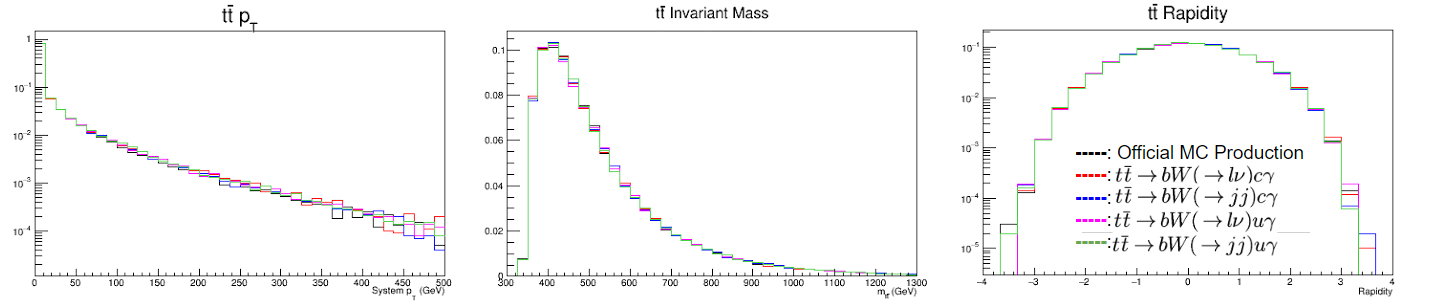
\includegraphics[width=\columnwidth]{../ThesisImages/FCNCValidation/ttBarSys.png}
	\caption{Normalized kinematics ($p_T$, $m_{t\bar{t}}$, and $y_{t\bar{t}}$) of the $t\bar{t}$ system produced by the model for each FCNC final state search and an official $t\bar{t}$ sample.
	}
	\label{fig:randomfinal2}
\end{figure}

\begin{figure}[h!]
	\centering
	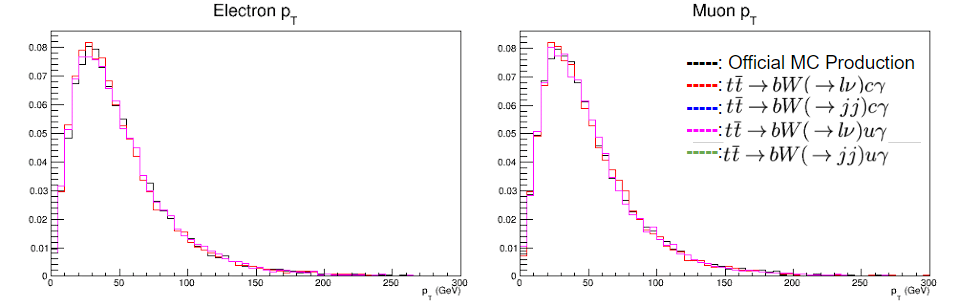
\includegraphics[width=\columnwidth]{../ThesisImages/FCNCValidation/lepton.png}
	\caption{Normalized $p_T$ of the electron and muons produced by the model for each FCNC final state search and an official $t\bar{t}$ sample.
	}
	\label{fig:LepVal}
\end{figure} 

The lepton validation plots in Figure \ref{fig:LepVal} only show events where the W is forced to decay leptonically as well as the official sample which does not have a preference for the final state decay, i.e., the W bosons are allowed to decay leptonically or hadronically.  
\begin{figure}[h!]
	\centering
	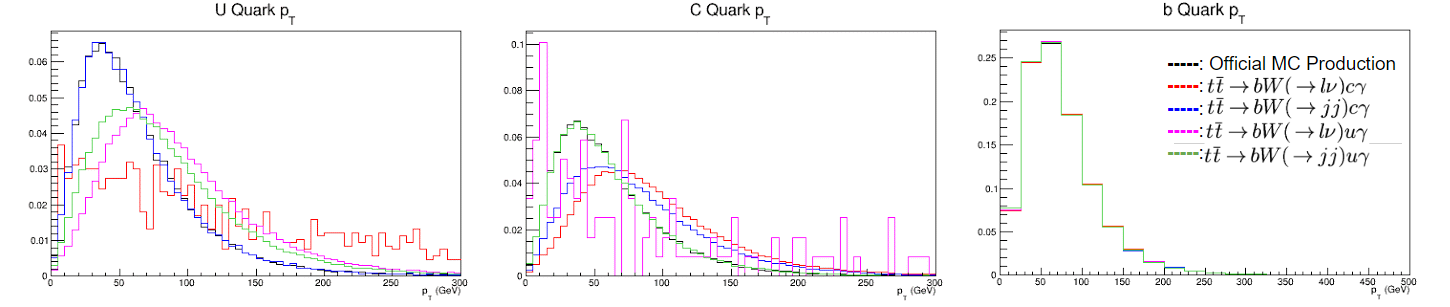
\includegraphics[width=\columnwidth]{../ThesisImages/FCNCValidation/quarks.png}
	\caption{Normalized $p_T$ of the up, charm, and bottom quarks produced by the model for each FCNC final state search and an official $t\bar{t}$ sample.
	}
	\label{fig:QuarkVal}
\end{figure}
No unexpected deviations from the Standard Model produced $t\bar{t}$ samples are seen in any of the validation plots.  The deviations seen in Figure \ref{fig:QuarkVal} are misplaced quarks from NLO processes.  The shifted mean values in the up and charm $p_T$ spectrum are also expected.  In those samples the up or charm quark is coming directly from the top quark as opposed to a W boson, which means it will have significantly boosted momentum.  The same boost holds for the photons as well, as shown in Figure \ref{fig:photonValidation}.

\begin{figure}[h!]
	\centering
	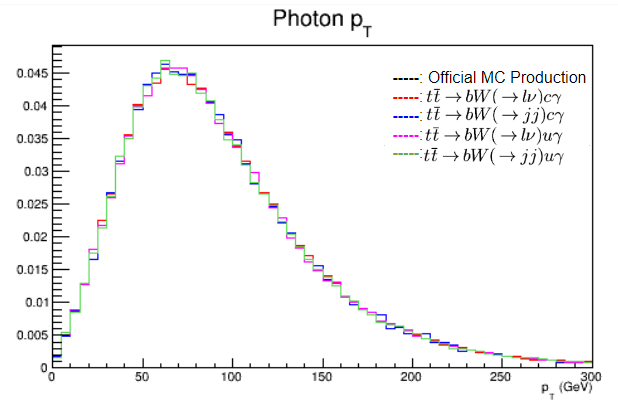
\includegraphics[width=.8\columnwidth]{../ThesisImages/FCNCValidation/photon.png}
	\caption{Normalized $p_T$ of the photons produced by the model for each FCNC final state search and an official $t\bar{t}$ sample.  There is 0 contribution from the official $t\bar{t}$ sample.
	}
	\label{fig:photonValidation}
\end{figure}

In the model there are left-and right-handed dipole moment couplings.  Investigation into differences between the kinematics of the quarks produced using each of these couplings is shown in Figure \ref{fig:LHRHcomp}.
\[ \mathcal{L}_{\gamma t c} = -e \bar{c} \frac{i\sigma^{\mu\nu}q_\nu}{m_t}(\lambda^L_{ct}P_L+\lambda^R_{ct}P_R )t A_\mu + h.c. \]

\begin{figure}[h!]
	\centering
	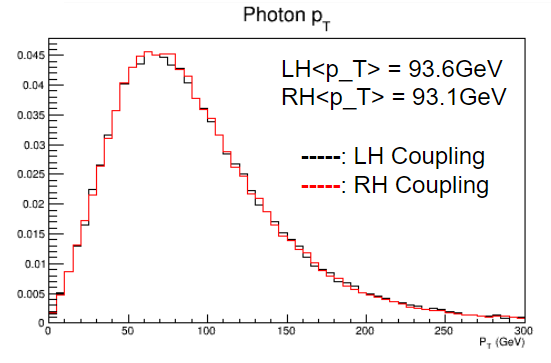
\includegraphics[width=.8\columnwidth]{../ThesisImages/FCNCValidation/PhotonLHRH.png}
	\caption{ Normalized $p_T$ of the photons produced by the model using the Left-handed (LH) and Right-handed (RH) couplings.
	}
	\label{fig:LHRHcomp}
\end{figure}

No differences in final state kinematics were shown in the right-handed coupling compared to the left-handed coupling.  Due to this, only one coupling value was used in the production.  In the end only leptonic decays of the W were produced officially.  The leptonic state is simpler to search for than a final state not involving leptons because of the much larger backgrounds from QCD processes.  The lepton offers many handles for searching for these rare FCNC decays.  While using the leptonic final state it is not necessary to use combinatorics for event reconstruction as each object is unique and comes from one particular object.  In this analysis the final state involves a light jet and a photon (from the FCNC decay), and a lepton, photon, and b-jet (from the Standard Model top decay).



%%%%%%%%%%%%%%%%%%%%%%%%%%

\section{Object Reconstruction}

After the events are simulated, or collected in case of real data, the collections of energy deposits within the detector systems must be transformed into meaningful physics objects through reconstruction.  Reconstruction is typically done in two major steps using the specialized detectors covered in Chapter \ref{ch:LHCDetector}.  The Inner Detector and Muon System turn patterns of hits within the tracking detectors into tracks that have direction and momentum information.  The calorimeter system transforms the energy deposits within the calorimeters into calibrated energy deposits with a particular position.  These tracks and calorimeter deposits are used to create physics objects (electrons, muons, etc.) by using particle identification techniques to reconstruct the underlying physics event.  For the analysis presented in this dissertation, the final state signal particles that need to be reconstructed are one lepton (an electron or a muon), one photon, two quarks (one light flavor and one b quark), and one neutrino (missing transverse energy as it is the only particle that does not interact with the detector).  Each of these particles has a particular signature in the subdetectors of the ATLAS detector, shown in Figure \ref{fig:ATLASInteractions}.

\begin{figure}[h]
	\centering
	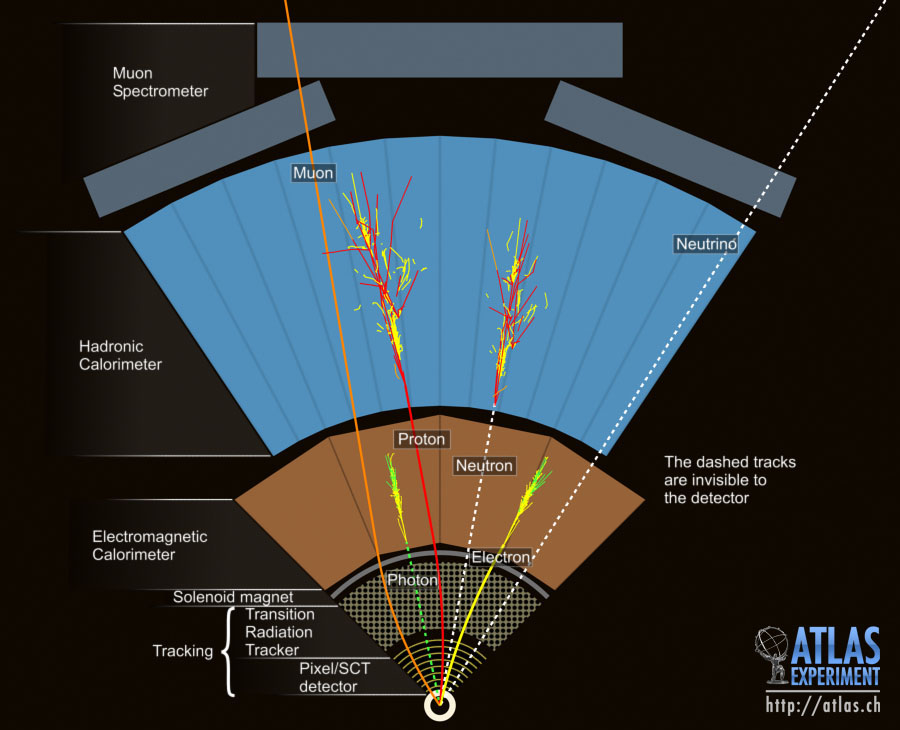
\includegraphics[width=\columnwidth]{../ThesisImages/Simulation/ParticleInteractions.jpg}
	\caption[Cross section of a simulated ATLAS detector showing how various particles interact with ATLAS subsystems.]{Cross section of a simulated ATLAS detector showing how various particles interact with ATLAS subsystems.  Solid lines indicate interactions while dashed lines indicate that no interactions typically occur in that section of the detector \cite{ParticleInteractions}.
	}
	\label{fig:ATLASInteractions}
\end{figure}


\subsection{Electrons}
Electrons interacting within the ATLAS detector leave a track in the Inner Detector as well as a cluster of energy in the electromagnetic calorimeter.  The track and cluster are required to be matched together to be identified as an electron candidate\cite{ElectronID}.  As electrons move through the detector they create electromagnetic showers through bremsstrahlung which can produce electron-positron pairs.  The process continues as the particles continue to give energy to the detector.  This collection of electrons, positrons, and photons creates a signature energy cluster in the calorimeter.  

Electron identification algorithms are applied to the electron candidates to separate prompt and isolated electron candidates from electrons that come from backgrounds such as converted photons and misidentified jets.  The electron idenification algorithms use a sliding window ($3\times5$ cells in $\eta \times \phi$ within the barrel region) in the high granularity section of the LAr electromagnetic calorimeter to search for electron cluster ``seeds'' greater than 2.5 GeV.  Clusters are created around these seeds to form the electromagnetic shower and remove possible duplicate electron signals by containing them within the cluster.  Further pattern recognition for the track fitting allows even larger amounts of energy into the shower to account for bremsstrahlung in the shower shape.  Tracks and clusters are then matched to give electron candidates.  

Electrons coming from background jets or photon conversion are called non-prompt as they do not originate from a signal object or the primary vertex.  In order to reject these electrons, other discriminating variables are used in addition to the track-cluster matching.  These variables include the amount of energy leakage into the hadronic calorimeter, the shower development throughout the electromagnetic calorimeter, and the amount of radiation measured in the TRT.  Three electron identification working points are used: Loose, Medium, and Tight.  Each of these operating points have their own level of background rejection and signal efficiency.  Working points with higher background rejection are a subset of those with lower background rejection.

Isolation variables are another useful tool in the identification of signal electrons from converted photons produced in hadron decays and light hadron misidentification.  These variables are defined by a cone size around the electron candidate and are the sum of the transverse variable (momentum or energy) of all of the tracks within the cone, $p_{T}^{\text{cone0.2}}$ with a cone of $\Delta R =0.2$ (or 10 GeV/$E_T$, for high energy electrons) and $E_{T, Topo}^{\text{varcone0.4}}$ with a cone defined in a similar manner.  

Because the LAr calorimeter is a sampling calorimeter, the energy deposits must be calibrated and scaled such that the true electron energy is read out and not just the small amount of energy deposited into the active layers as discussed in Section \ref{sec:EMHCal}.  The energy scale is calibrated to be uniform throughout the detector.  Any residual differences between data and simulation are corrected.  The calibration strategy was developed for optimal performance in LHC Run-1\cite{ElectronCalib1} and updated for the conditions of LHC Run-2\cite{ElectronCalib2}.

\subsection{Muons}
Muons behave differently from other particles as they traverse the detector.  They act as minimum-ionizing particles (MIPs) throughout the calorimeter.  The Muon Spectrometer (MS), Section \ref{sec:MuCal}, specializes in precision measurements of muons.  The Inner Detector (ID) plays a pivotal role in the identification of muons as it offers an independent measure of the muon characteristics.  The muon reconstruction process uses a specific set of variables as well\cite{MuonID}.  These variables include: \textit{ q/p significance}: the difference in the ratio of track charge and momentum measured with the ID and MS, $\rho'$: the difference between the transverse momenta measured with the ID and MS, and $\chi^2$ of the combined track fit using tracks from both the ID and MS.

Muons are separated out into four separate types depending on their interactions with the various subdetectors.  The best muon candidates are combined muons that use hits in the MS to trace back to a track in the ID in order to reconstruct the entire muon track.  Segment-tagged muons are muon candidates that leave a track in the ID but only a segment in the MS instead of a full track.  Segment-tagged muons can occur because of the muon having low $p_T$ or crossing through a region of the MS with reduced acceptance.  Extrapolated muons require only tracks in the MS and are used in regions of $\eta, \phi$ phase space that the ID does not cover.  Calorimeter-tagged muons are muons identified by MIPs in the calorimeters and are used to find muons that cross the ID and MS in regions where cabling might prevent particle detection.

Muons also have their own set of isolation criteria which is track-based $p_{T}^{\text{varcone0.3}}$, with a cone of $\Delta \text{R} = \text{min}(0.3,10\text{ GeV}/p_T)$.  As with electrons, various working points are available at the analysis level for muons.  These working points are named similarly: Loose, Medium, Tight, and High-$p_T$ in order of background rejection.  

High-$p_T$ jets that punch through the hadronic calorimeter can leave tracks in the MS which could be identified as muons.  These would be identified as a bad or a fake muon because of the high-hit multiplicities they leave in the MS as opposed to a single track left by a muon as it is a MIP.  Another source of bad muons is a mismeasured ID track that gets incorrectly matched to segments in the MS.  Fake muons are a source of fake missing transverse energy, $ \slashed{E}_T$

\subsection{Photons}
Photons behave very similarly to electrons in the calorimeter in that they also produce an electromagnetic shower in the calorimeter.  However, they are neutrally charged particles meaning that they should not leave a track in the ID as they do not bend and produce bremsstrahlung photons traveling through the magnetic field.  Prompt photons pair-produce electrons in the tracker, but this process can be identified by using the associated cluster in the electromagnetic calorimeter if it is matched to two tracks with opposite charge.  This process produces what is called a converted photon.  Unconverted photons have no matching tracks associated with an electromagnetic cluster.   

\begin{center}
\begin{table}
\noindent\makebox[\textwidth]{%
\small
{\renewcommand{\arraystretch}{1.6}
\begin{tabularx}{1.25 \textwidth}{ l X lll }
\hhline{=====}
Category 	& Description  & Name  & \textit{loose}  & \textit{tight} \\ \hline
Acceptance 	& $|\eta|<2.37$, with $1.37 \leq |\eta|<1.52$ excluded  & -  &  \checkmark  & \checkmark \\
Hadronic Leakage & Ratio of $E_T$ in the first sampling layer of the hadronic calorimeter to $E_T$ of the EM cluster (used over the range $0.8<|\eta|$ or $|\eta|>1.52$) & $R_{\text{had}_1}$  &  \checkmark  &  \checkmark \\
		&  Ratio of $E_T$ in the hadronic calorimeter to $E_T$ of the EM cluster (used over the range $0.8<|\eta|<1.37$) & $R_{\text{had}}$  &   \checkmark &  \checkmark \\
EM Middle Layer & Ratio of the energy in $3\times 7$ $\eta \times \phi$ cells over the energy in $7\times 7$ cells centered around the photon cluster position & $R_{\eta}$ &   \checkmark &  \checkmark \\
		 & Lateral shower width, $\sqrt{(\Sigma E_{i} \eta_{i}^2 )/(\Sigma E_i )-((\Sigma E_i \eta_i )/(\Sigma E_i))^2}$, where $E_i$ is the energy and $\eta_i$ is the pseudorapidity of cell i and the sum is calculated within a window of $3\times 5$ cells & $\omega_{\eta_2}$ &  \checkmark &   \checkmark\\
		 & Ratio of the energy in $3 \times 2$ $\eta \times \phi$ strips, over the energy of $3\times 6$ cells centered around the photon cluster position  & $R_\phi$ &  &  \checkmark \\
EM Strip Layer & Lateral shower width, $\sqrt{(\Sigma E_i (i-i_\text{max})^2)/(\Sigma E_i)}$, where i runs over all strips in a window of $3 \times 2$ $\eta \times \phi$ strips, and $i_{\text{max}}$ is the index of the highest-energy strip calculated from three strips aroudn the strip with maximum energy deposit & $\omega_{s\text{ 3}}$  &  & \checkmark \\
		 & Total lateral shower width  $\sqrt{(\Sigma E_i (i-i_\text{max})^2)/(\Sigma E_i)}$, where i runs over all strips in a window of $20 \times 2$ $\eta \times \phi$ strips, and $i_{\text{max}}$ is the index of the highest-energy strip measured in the strip layer & $\omega_{s\text{ tot}}$  &  &  \checkmark \\
		 & Energy outside the core of the three central strips but within seven strips divided by energy within the three central strips  & $f_\text{side}$ &  &  \checkmark  \\
		 & Difference between the energy associated with the second maximum in the strip layer and the energy reconstructed in the strip with the minimum value found between the first and second maxima & $\Delta E_s$ &  &   \checkmark \\
		 & Ratio of the energy difference between the maximum energy deposit and the energy deposit in the secondary maximum in the cluster to the sum of these energies & $E_\text{ratio}$ &  &  \checkmark \\
		 & Ratio of the energy in the first layer to the total energy of the EM cluster & $f_1$ &  &  \checkmark \\
\hhline{=====}
\end{tabularx}
\normalsize
}}
\caption[Photon identification variables used for \textit{loose} and \textit{tight} photon identification.]{Photon identification variables used for \textit{loose} and \textit{tight} photon identification, taken from \cite{PhotonID}.}
\label{tab:PhotonVars}
\end{table}
\end{center}

Prompt photons produce narrower energy deposits in the electromagnetic calorimeter and have smaller leakage into the hadronic calorimeter compared to background photons.  The energy contained within narrow structure in $\eta \times \phi$ strips compared to the energy contained in a larger section can help identify prompt from non-prompt photons\cite{PhotonID}.  Cuts on this and the other variables listed in Table \ref{tab:PhotonVars} are tuned to reduce dependency of identification efficiency on the pile-up conditions of Run-2.


\subsection{Jets}

Contrasting with electromagnetic showers produced by electrons and photons, hadronic showers form through QCD processs.  Quarks very quickly undergo showering by emitting gluons which further produce quark-antiquark pairs, analogous to the photons and pair-produced electron-positron pairs of electromagnetic showers.   When quarks have enough energy they hadronize by producing bound states of particles.  These particles are typically pions or mesons that are measured by the ATLAS detector.  The top quark is the only quark that decays before hadronization because it decays so fast ($5\times10^{-25}$ s).  The spray of hadrons coming from a quark from the initial interaction is called a jet and is a collection of detector objects that are traced back and assigned to the quark(s) in the final state of the interaction.  These algorithms are called jet-finding algorithms.  Pictoral representations of the same event reconstructed with four various algorithms is shown in Figure \ref{fig:VarJetAlgs}.

%Ben\cite{CambridgeAachen}
%Ben\cite{JetCleaning}
\begin{figure}[h!]
	\centering
	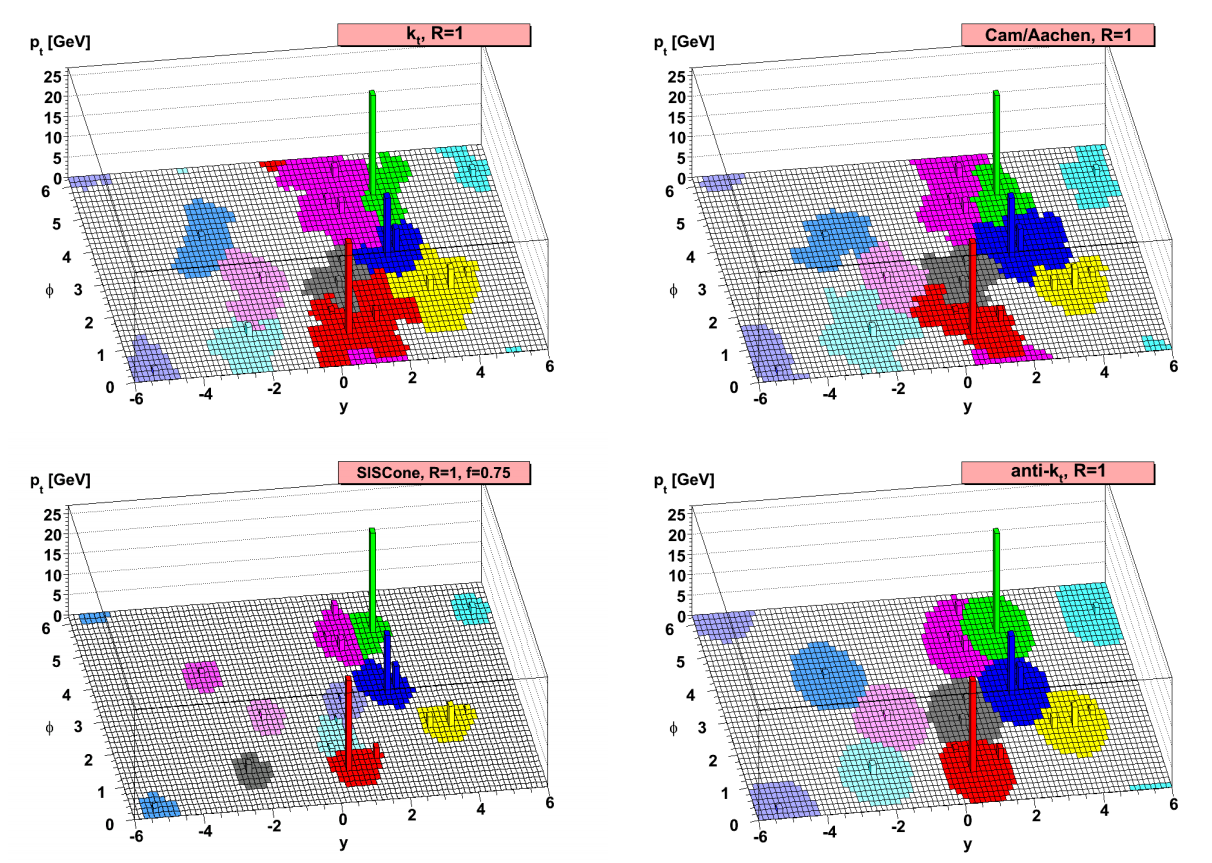
\includegraphics[width=\columnwidth]{../ThesisImages/Simulation/VarJetAlgs.png}
	\caption[A sample parton-level event with many random soft jet objects, clustered with four different jets algorithms, illustrating the areas of the resulting hard jets. For kt and Cambridge/Aachen the detailed shapes are in part determined by the specific set of ghosts used, and change when the ghosts are modified.]{A sample parton-level event with many random soft jet objects, clustered with four different jets algorithms, illustrating the areas of the resulting hard jets. For kt and Cambridge/Aachen the detailed shapes are in part determined by the specific set of ghosts used, and change when the ghosts are modified\cite{antikt}. 
	}
	\label{fig:VarJetAlgs}
\end{figure}

The jets in this analysis use the anti-$k_T$ algorithm\cite{antikt} with a radius parameter $R=0.4$.  Jets are collections of clustered particles whose properties are dependent on the algorithm used to reconstruct them.  How they are defined can change the physics objects that are eventually analyzed.  The anti-$k_T$ algorithm is preferred because it is infrared and collinear safe.  Infrared-safe jet algorithms do not merge two jets with a soft emission between them.  Adding or removing a soft term between two jets should not change which objects are called jets.  Collinear safe jet algorithms do not change the jet collection if the high transverse momentum particles are split or merged.  Another added benefit of the anti-$k_T$ jet-finding algorithm is that it produces roughly circular jet objects, thereby simplifying the calculation of the energy density and simplifying the calibration of the jet object.

The anti=$k_T$ algorithm calculates the distance between an object $i$ and all possible jet objects $j$ ($d_{ij}$) and the beam ($d_{iB}$)
\[ d_{ij} = \text{min}(k_{ti}^{2p},k_{tj}^{2p})\frac{\Delta^2_{ij}}{R},\qquad 
d_{iB} = k_{ti}^{2p} \] 
where $k_{ti}$ is the transverse momentum, $\Delta$ is the distance between the objects, and $p=-1$.  This is a general form for the type of algorithm where the inclusive $k_T$ algorithm has a $p$ value of 1 and the inclusive Cambridge/Aachen algorithm has a $p$ value of 0 \cite{CambridgeAachen}.  The algorithm then follows that if $d_{ij}$ is smaller than $d_{iB}$ then objects $i$ and $j$ are merged, otherwise $i$ is labeled as a jet and removed from the list of entries of possible jet objects.  This is repeated for all entries in the list of possible jet objects.

Jet cleaning is also applied to remove events with jets built from known noisy parts of the calorimeter due to particular calorimeter cells or non-collision background in those areas\cite{JetCleaning}.  The fraction of events removed by the jet-cleaning process is negligible and should not lead to any significant measurement inefficiencies, a maximum of 0.015\% of the total events.  To reduce selecting jets that originate from pile-up interactions, another requirement on the jet object is made on the jet vertex tagger\cite{JetJVT, JetCleanTwiki} as follows:
\begin{enumerate}
\item For jets with $20 \mathrm{ GeV } < p_{T} < 60 \mathrm{ GeV }$ and $|\eta| < 2.4$: if any jet is bad AND that jet is not marked as pile-up by JVT, then reject the event.
\item For jets with $20 \mathrm{ GeV } < p_{T} < 60 \mathrm{ GeV }$ and $|\eta| \geq 2.4$: if any jet is bad, then reject the event.
\item For jets with $p_{T} \geq 60 \mathrm{ GeV }$: if any jet is bad, then reject the event.
\end{enumerate}


\subsubsection{B-Jets}

While jets originate from any quark, jets coming from b quarks can be identified due to their decay products.  B quarks hadronize into b-hadrons which have a relatively long lifetime compared to many other hadrons produced from light quarks.  The longer lifetime and the relativistic speeds at which the hadrons travel mean the particle travels a measurable distance before it decays ($400-500 \mu m$)\cite{CMSct}.  For b quarks resulting from top decays the boost they have is greater which leads to a larger decay distance.  A b-hadron with an average momentum of around 60 GeV will have a $c\tau$ of about 6 mm.  Thus, the vertex reconstructed from the energy coming from a b-hadron decay can be traced back to a point that does not correspond to the primary vertex of the event.    A pictoral representation of a b quark decay is shown in Figure \ref{fig:BTagVars}.  The b-jet vertex is called the secondary vertex.  

\begin{figure}[h!]
	\centering
	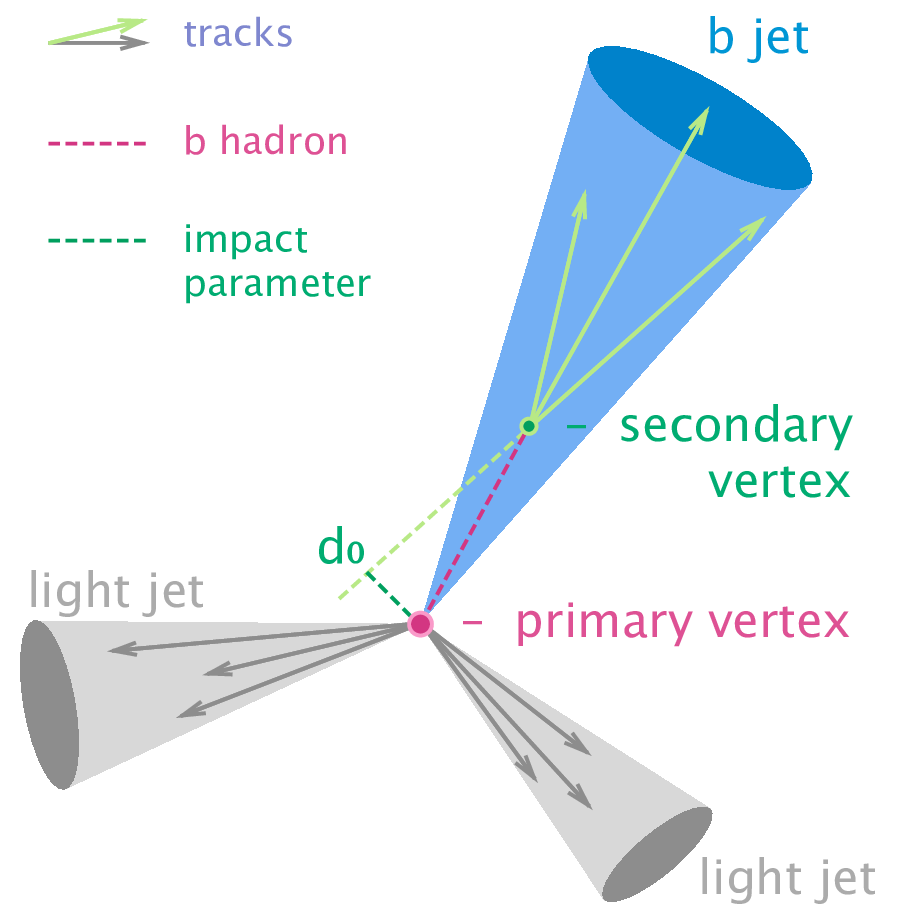
\includegraphics[width=.5\columnwidth]{../ThesisImages/Simulation/B-tagging_diagram.png}
	\caption[Pictoral representation of an event with a b-jet showing the secondary vertex and impact parameter.]{Pictoral representation of an event with a b-jet showing the secondary vertex and impact parameter\cite{BTagImg}. 
	}
	\label{fig:BTagVars}
\end{figure}

In addition to the secondary vertex, other variables are helpful in identifiying jets coming from b quarks.  By back tracing the tracks within the displaced vertex the minimum distance between the track and the interaction point can be measured, and is known as the impact parameter.  Reconstructing the decay chain of the jet is also used in determining the providence of the jet.  This information is used in a multivariate analysis (MVA) to identify jets coming from b quarks and reject jets coming from light quarks.

The MVA used in this analysis is the MV2c10, the discriminant used for b-jet identification\cite{BJet1718}.  The output distributions for various flavors of jets as well as background rejection and signal efficiency plots are shown in Figure \ref{fig:BTag}.  The c10 in the algorithm name refers to the background training sample of the MVA consisting of a 10\% fraction of c-jets.  The 77\% efficiency fixed-cut working point for b-jet identification was chosen for this analysis and is discussed in Section \ref{sec:NN}.  Differences in efficiency of b-tagging between data and simulation are taken into account with working point specific scale factors provided by the ATLAS Flavour Tagging Combined Performance group.

\begin{figure}[h!]
	\centering
	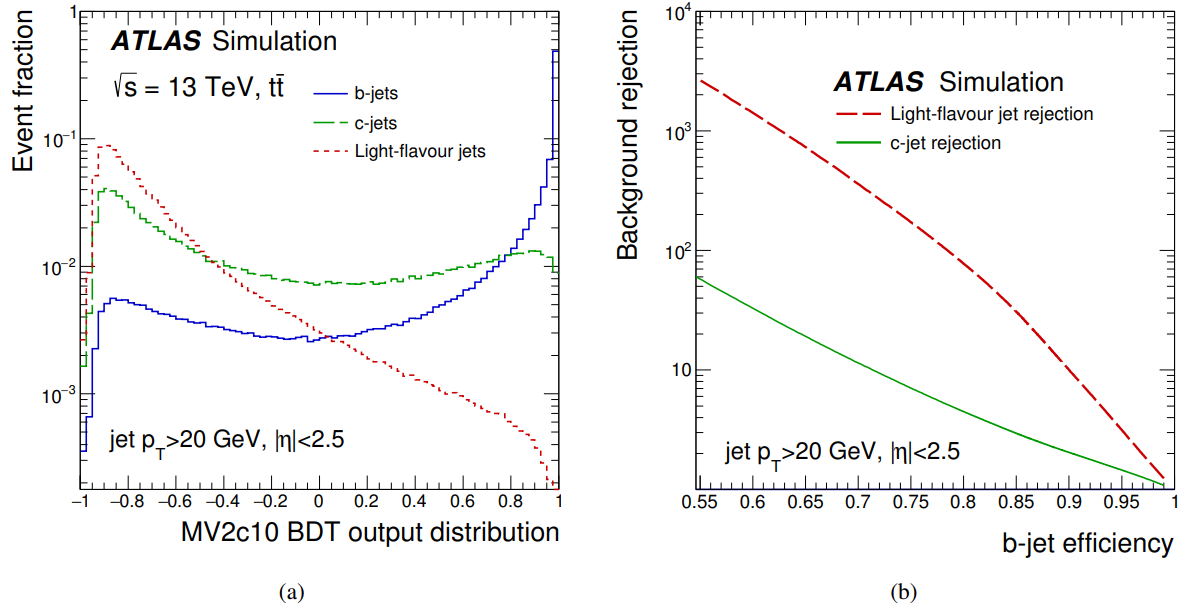
\includegraphics[width=\columnwidth]{../ThesisImages/Simulation/BTagMV2c10andRejVsEff.png}
	\caption[The MV2c10 output for b, c, and light flavored jets in simulated $t\bar{t}$ and the background rejection as a function of the b-jet efficiency.]{The MV2c10 output for b, c, and light flavored jets in simulated $t\bar{t}$ and the background rejection as a function of the b-jet efficiency\cite{BJetMVA}.
	}
	\label{fig:BTag}
\end{figure}


%\cite{Takubo:2017wvt}%IBL Preformance
\label{sec:bjetReco}

\subsection{Missing Transverse Energy}
The remaining signal object that has yet to be discussed is the neutrino coming from the W boson decay.  Neutrinos do not interact with the detectors as they pass through the ATLAS detector.  The only way to measure any properties of the neutrino in ATLAS events is to use conservation of momentum.  As previously mentioned the collision energy is unknown as partons do not carry a consistent fraction of the beam proton energy.  However, in the transverse plane to the beamline the total momentum is known to be very small.  Before the collision there is little beam divergence, on the order of 1 GeV of momentum in the transverse plane.  Therefore, the total transverse momentum of the collision products should be approximately zero.

Any imbalance in the momentum is referred to as Missing Transverse Momentum ($\slashed{E}_T$).  The negative vector sum of all reconstructed objects plus an additional soft term are used to calculate the missing energy in the x-plane and the y-plane\cite{METreco}.  A magnitude and an aziumuthal angle are calculated to give the \textbf{$\slashed{E}_T$} vector in the transverse plane, but this does not directly correspond to a neutrino which also has a momentum in the z direction.

\subsubsection{Neutrino Reconstruction}
In this analysis the signal contains only one source of missing energy, therefore all of the missing energy can be used to reconstruct a neturino object.  There is an ambiguity in the choice of the neutrino z-momentum.  To find the z-momentum a $\chi^2$ minimization is done:
\[ \chi^2 = \chi_{\text{SMTop}}^2 + \chi_{\text{W}}^2 \]
\[ \chi^2 = \frac{(m_{\text{bjet},l,\nu}-m_t)^2}{\sigma_{\text{SMTop}}^2} + \frac{(m_{l,\nu}-m_W)^2}{\sigma_W^2}. \]
The widths $\sigma_{\text{SMTop}}$ and $\sigma_W^2$ are determined from signal Monte Carlo.  The event objects are combined to calculate the invariant mass of the top quark (the combination of the b-jet, lepton, and neutrino) and the W boson (combination of the lepton and neutrino).  The $\chi^2$ minimization is done while varying the z-momentum of the neutrino.  The neutrino momentum that corresponds to the smallest $\chi^2$ value is assigned to the neutrino object for further use in the analysis.  The $\chi^2$ values are also used as a discriminating variable and fed into a neural network (Section \ref{sec:NN}).







